\chapter{Conceptual Model}

\section{Introduction}
	The conceptual model illustrates through mock ups how the system will appear to different actors who might use the system. The webpage will look the same overall, however it has small differences between users who decide to create an account and users who don’t have an account.  Figure 5.1 shows the overall view. This remains the same for both users and it is what a user sees from a cold start. Figure 5.2 shows the user login and registration page. Figure 5.3 shows the user customization page. Here a user can select the teams he or she is interested in. Figure 5.4 shows what the screen looks like after a user has logged in.

\section{Landing Page}
\begin{figure}[!ht]
      \centering
      \fbox {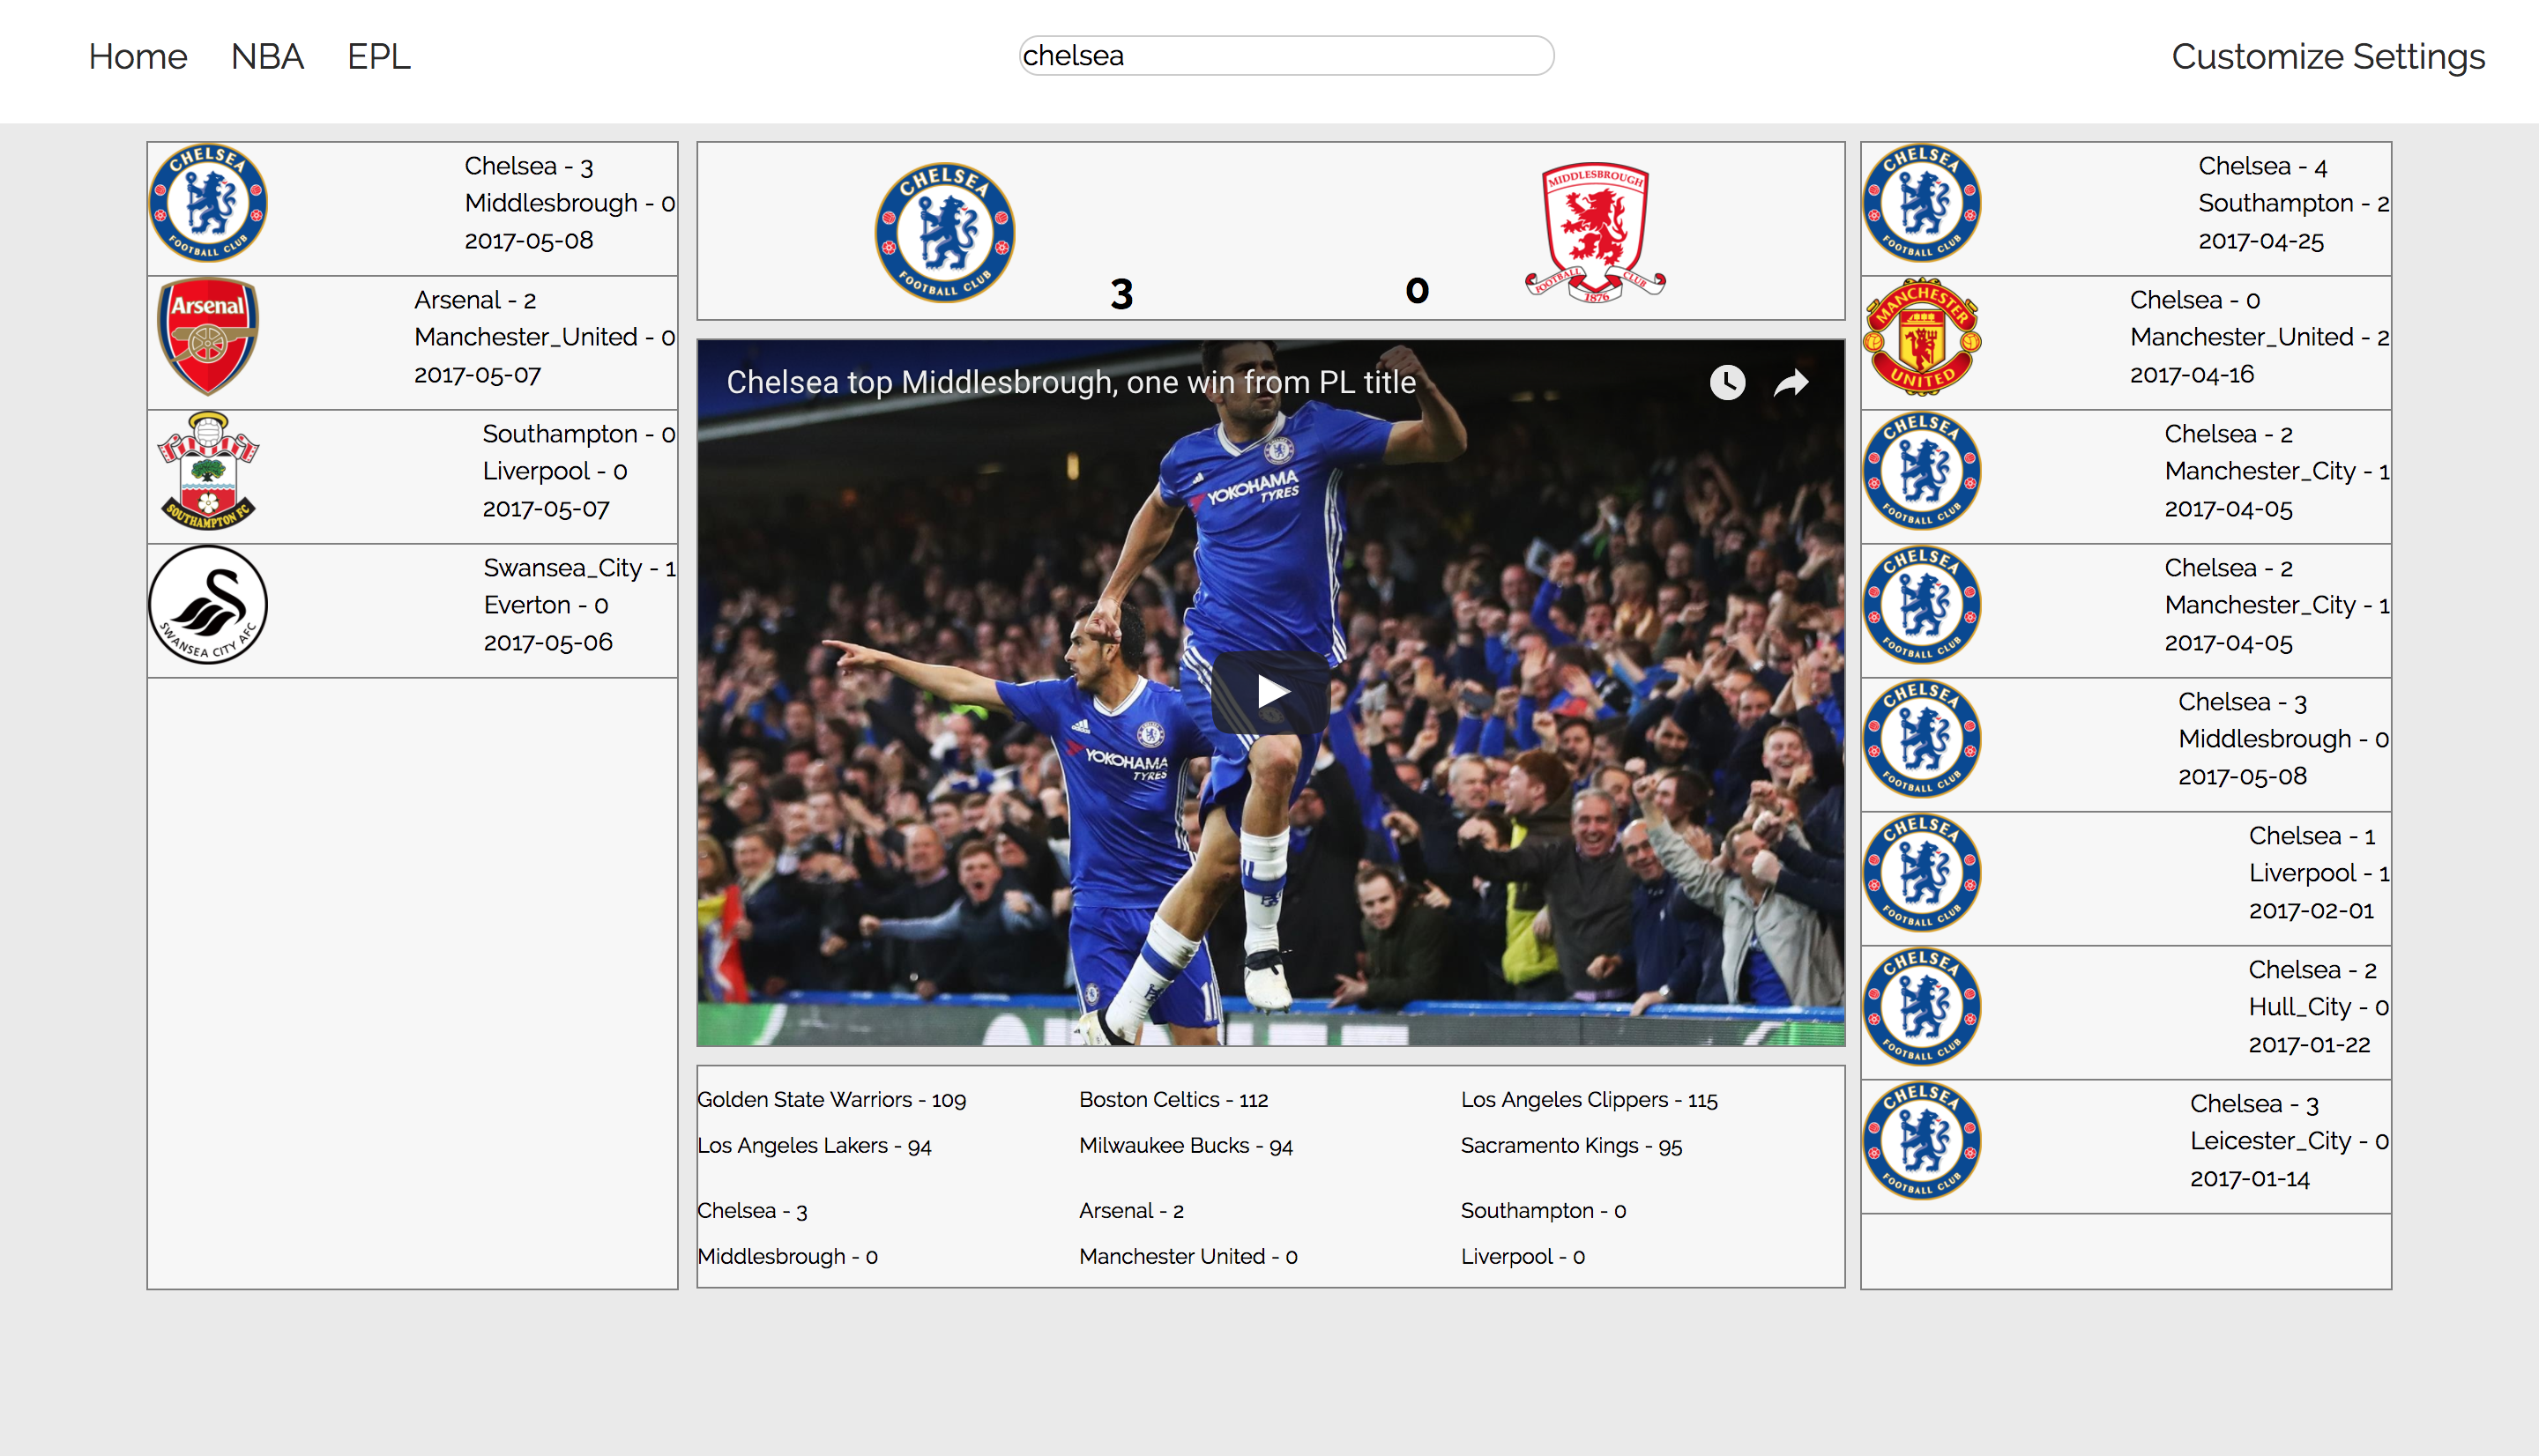
\includegraphics[scale=0.25]{landing.png}}
      \caption{Overall view of website as guest}	
\end{figure}

\section{User Login/Registration Page}
\begin{figure}[!ht]
      \centering
      \fbox {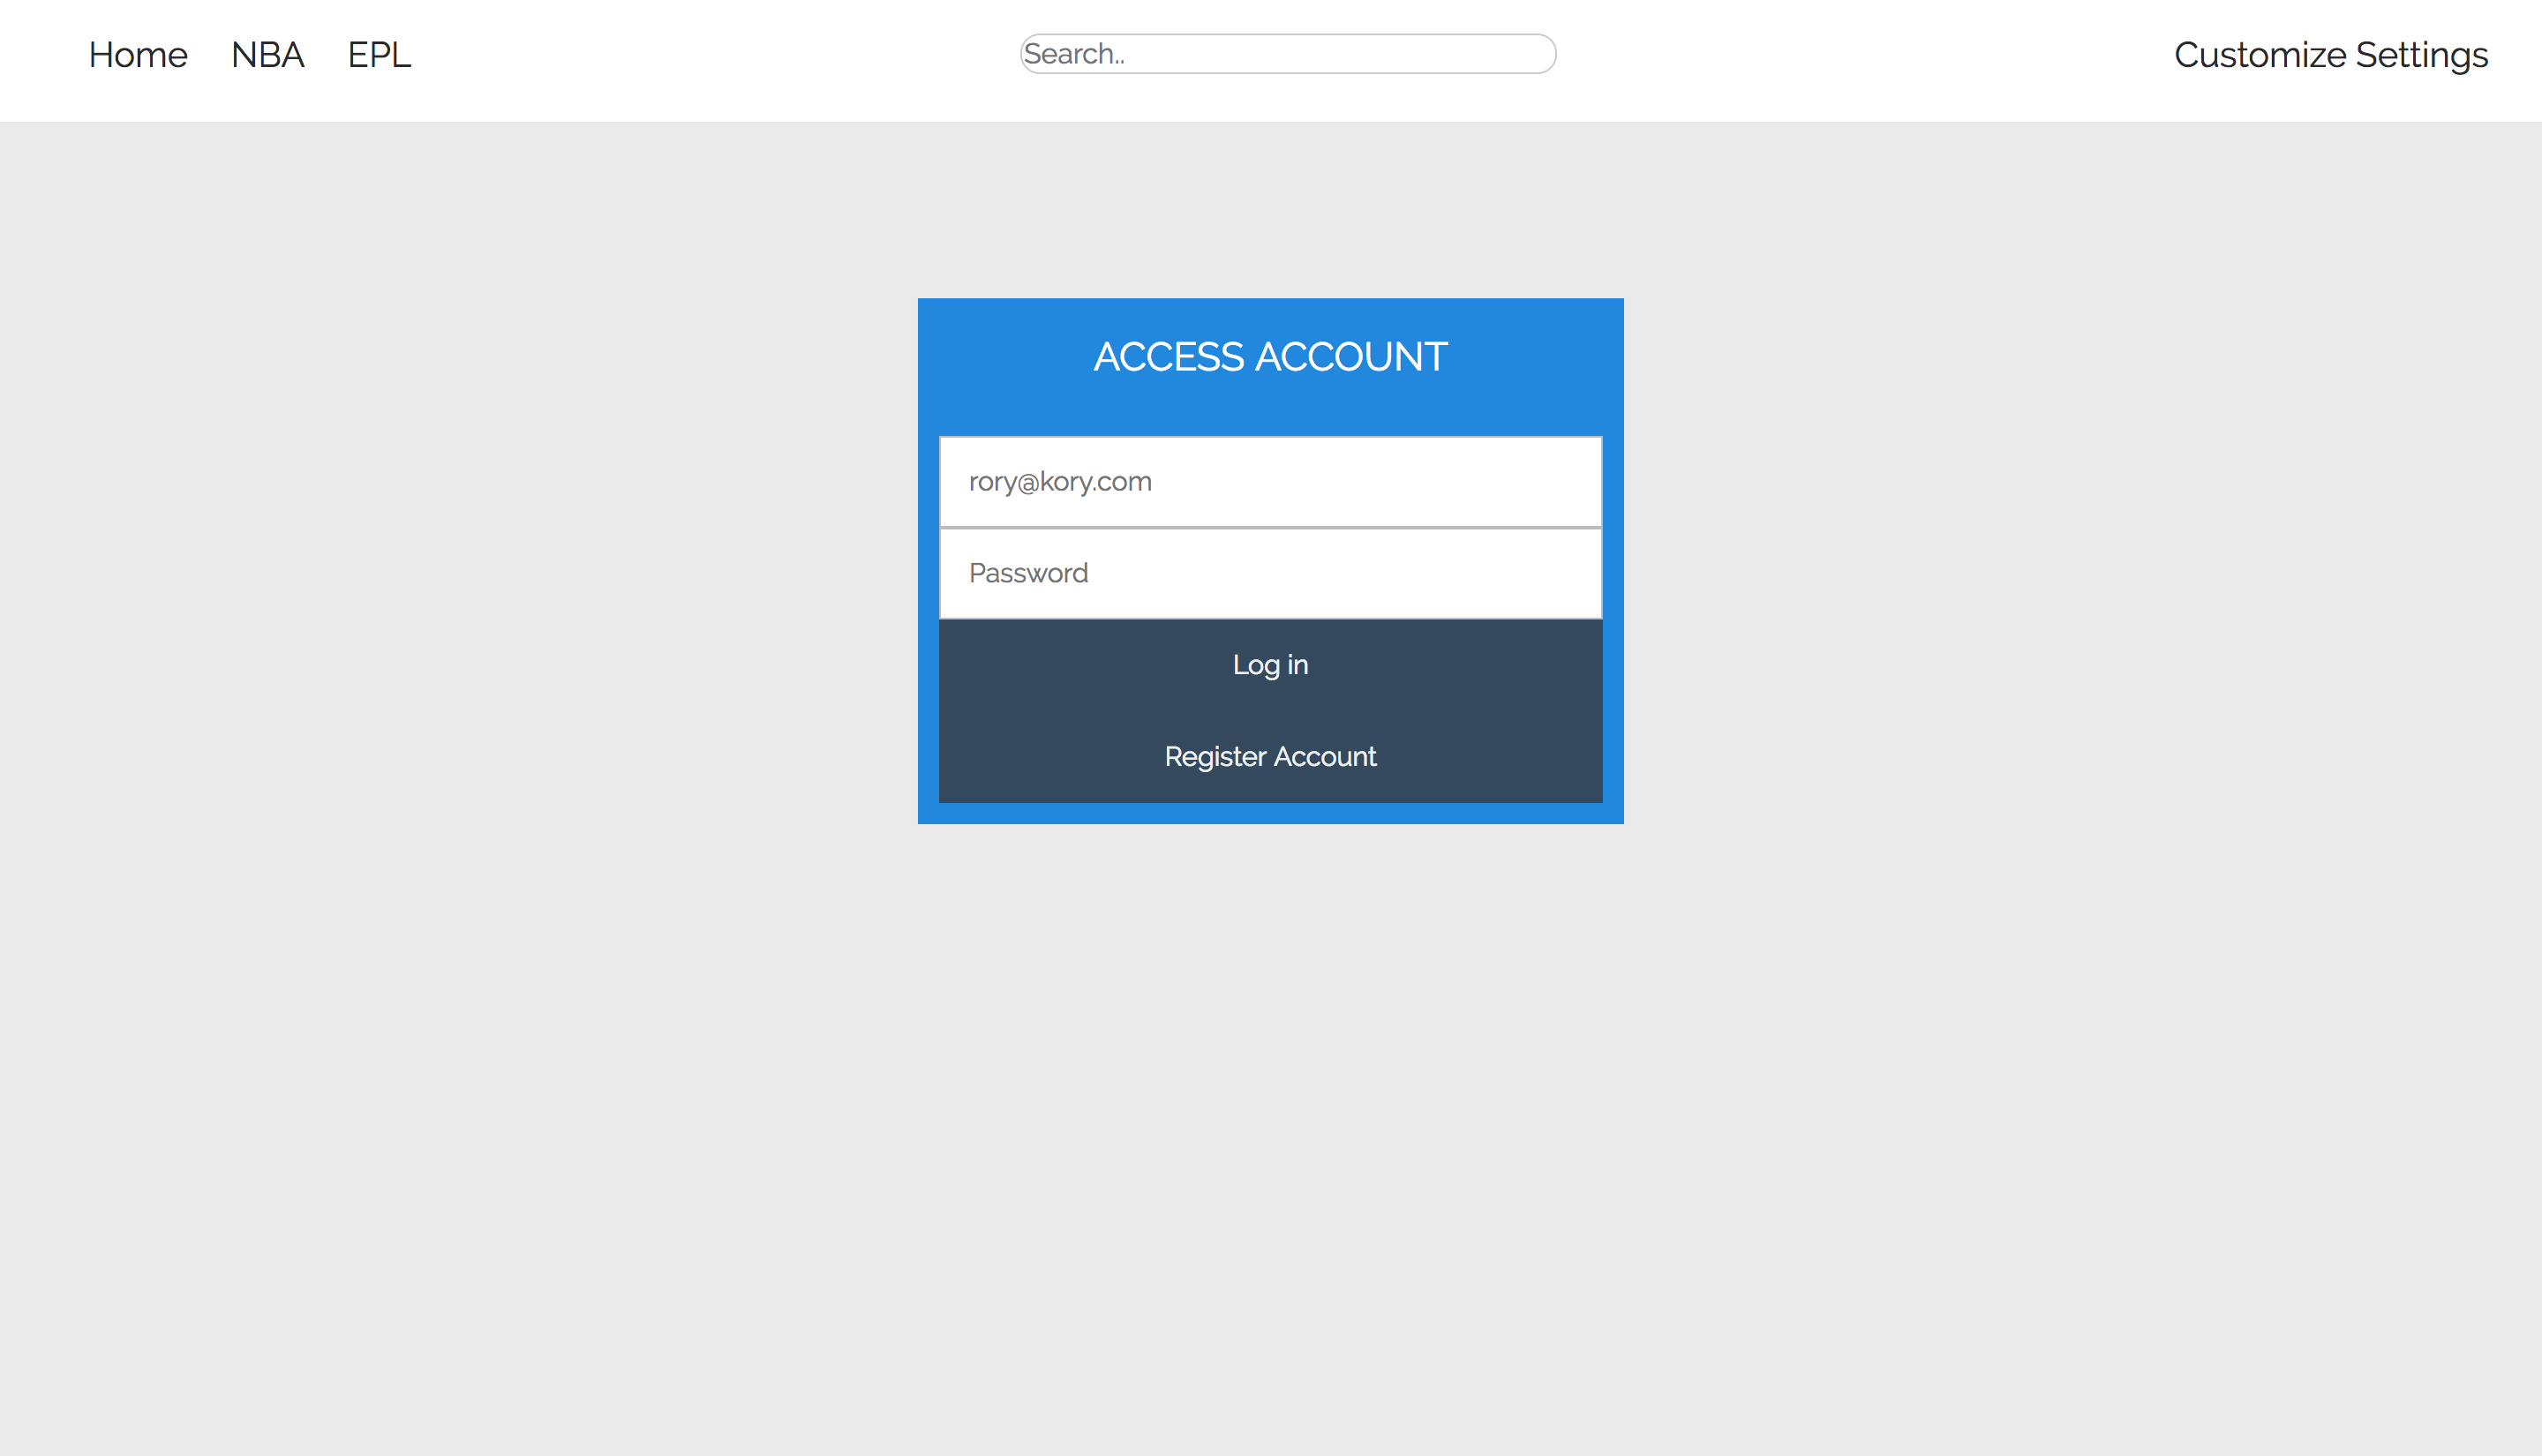
\includegraphics[scale=0.25]{signin.png}}
      \caption{Account creation}	
\end{figure}

\section{User Customization Page}
\begin{figure}[!ht]
      \centering
      \fbox {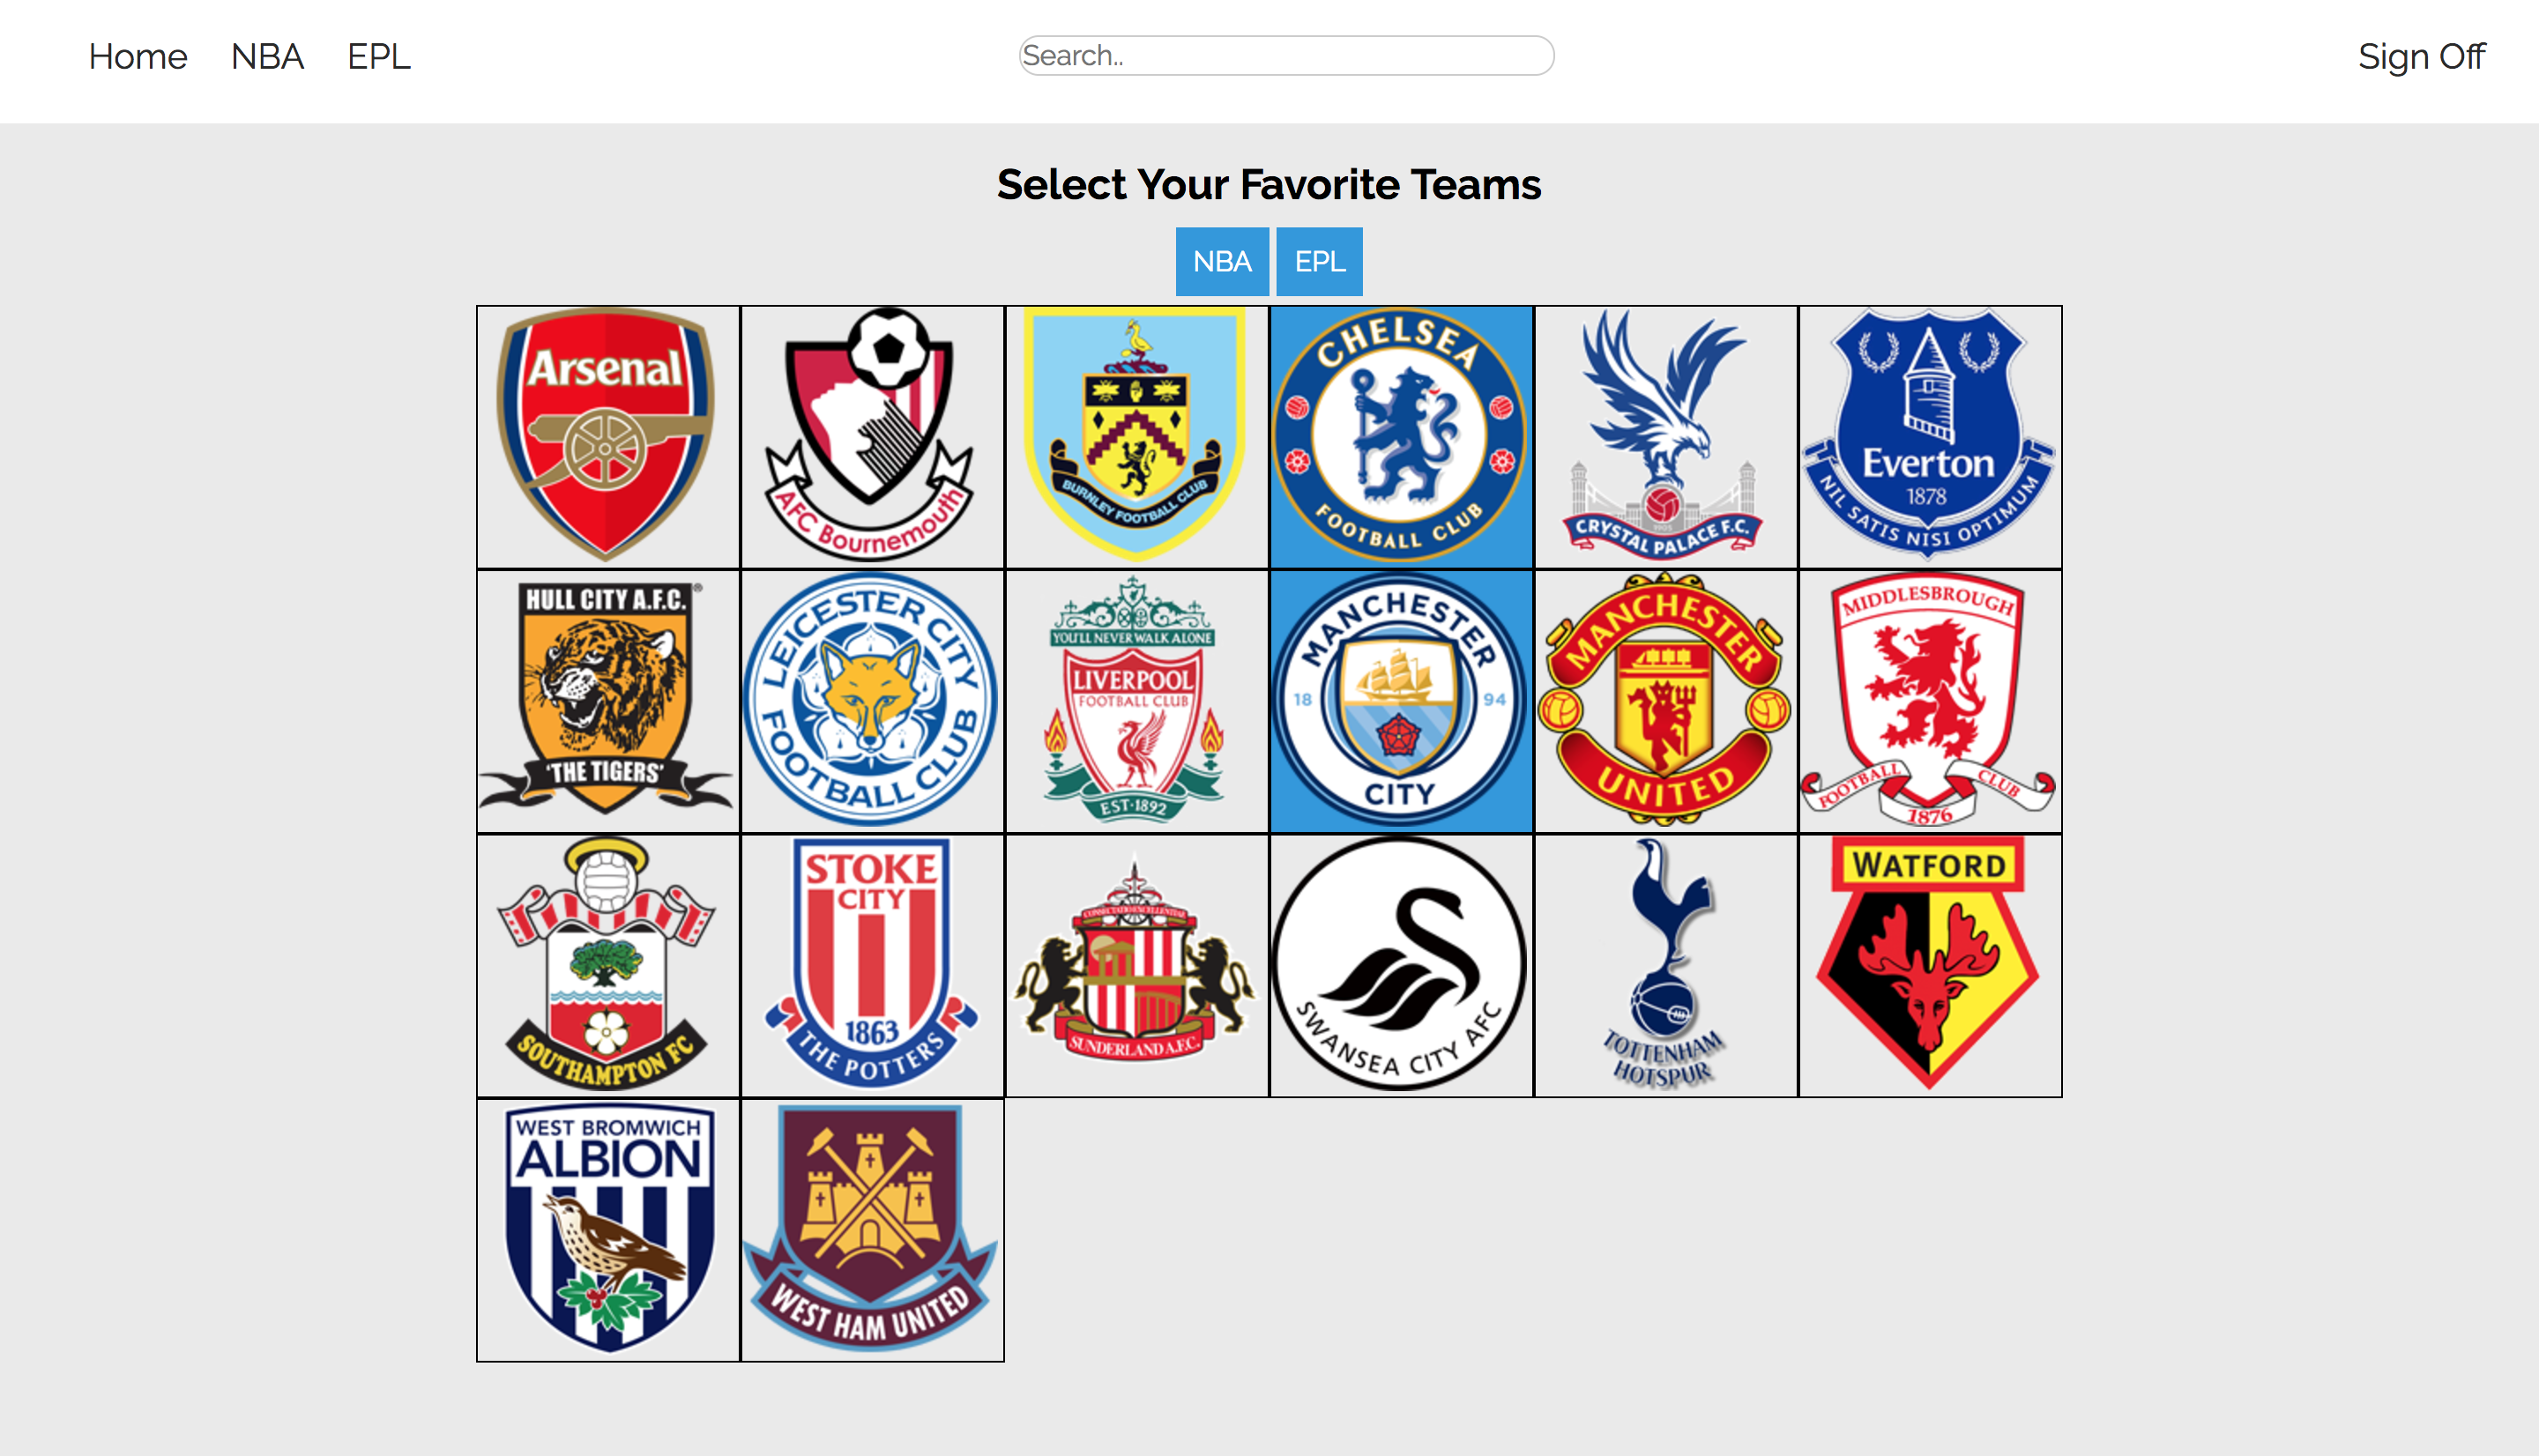
\includegraphics[scale=0.25]{register.png}}
      \caption{User customization of favorite EPL soccer teams}	
\end{figure}

\newpage
\section{Logged-In User Page}
\begin{figure}[!ht]
      \centering
      \fbox {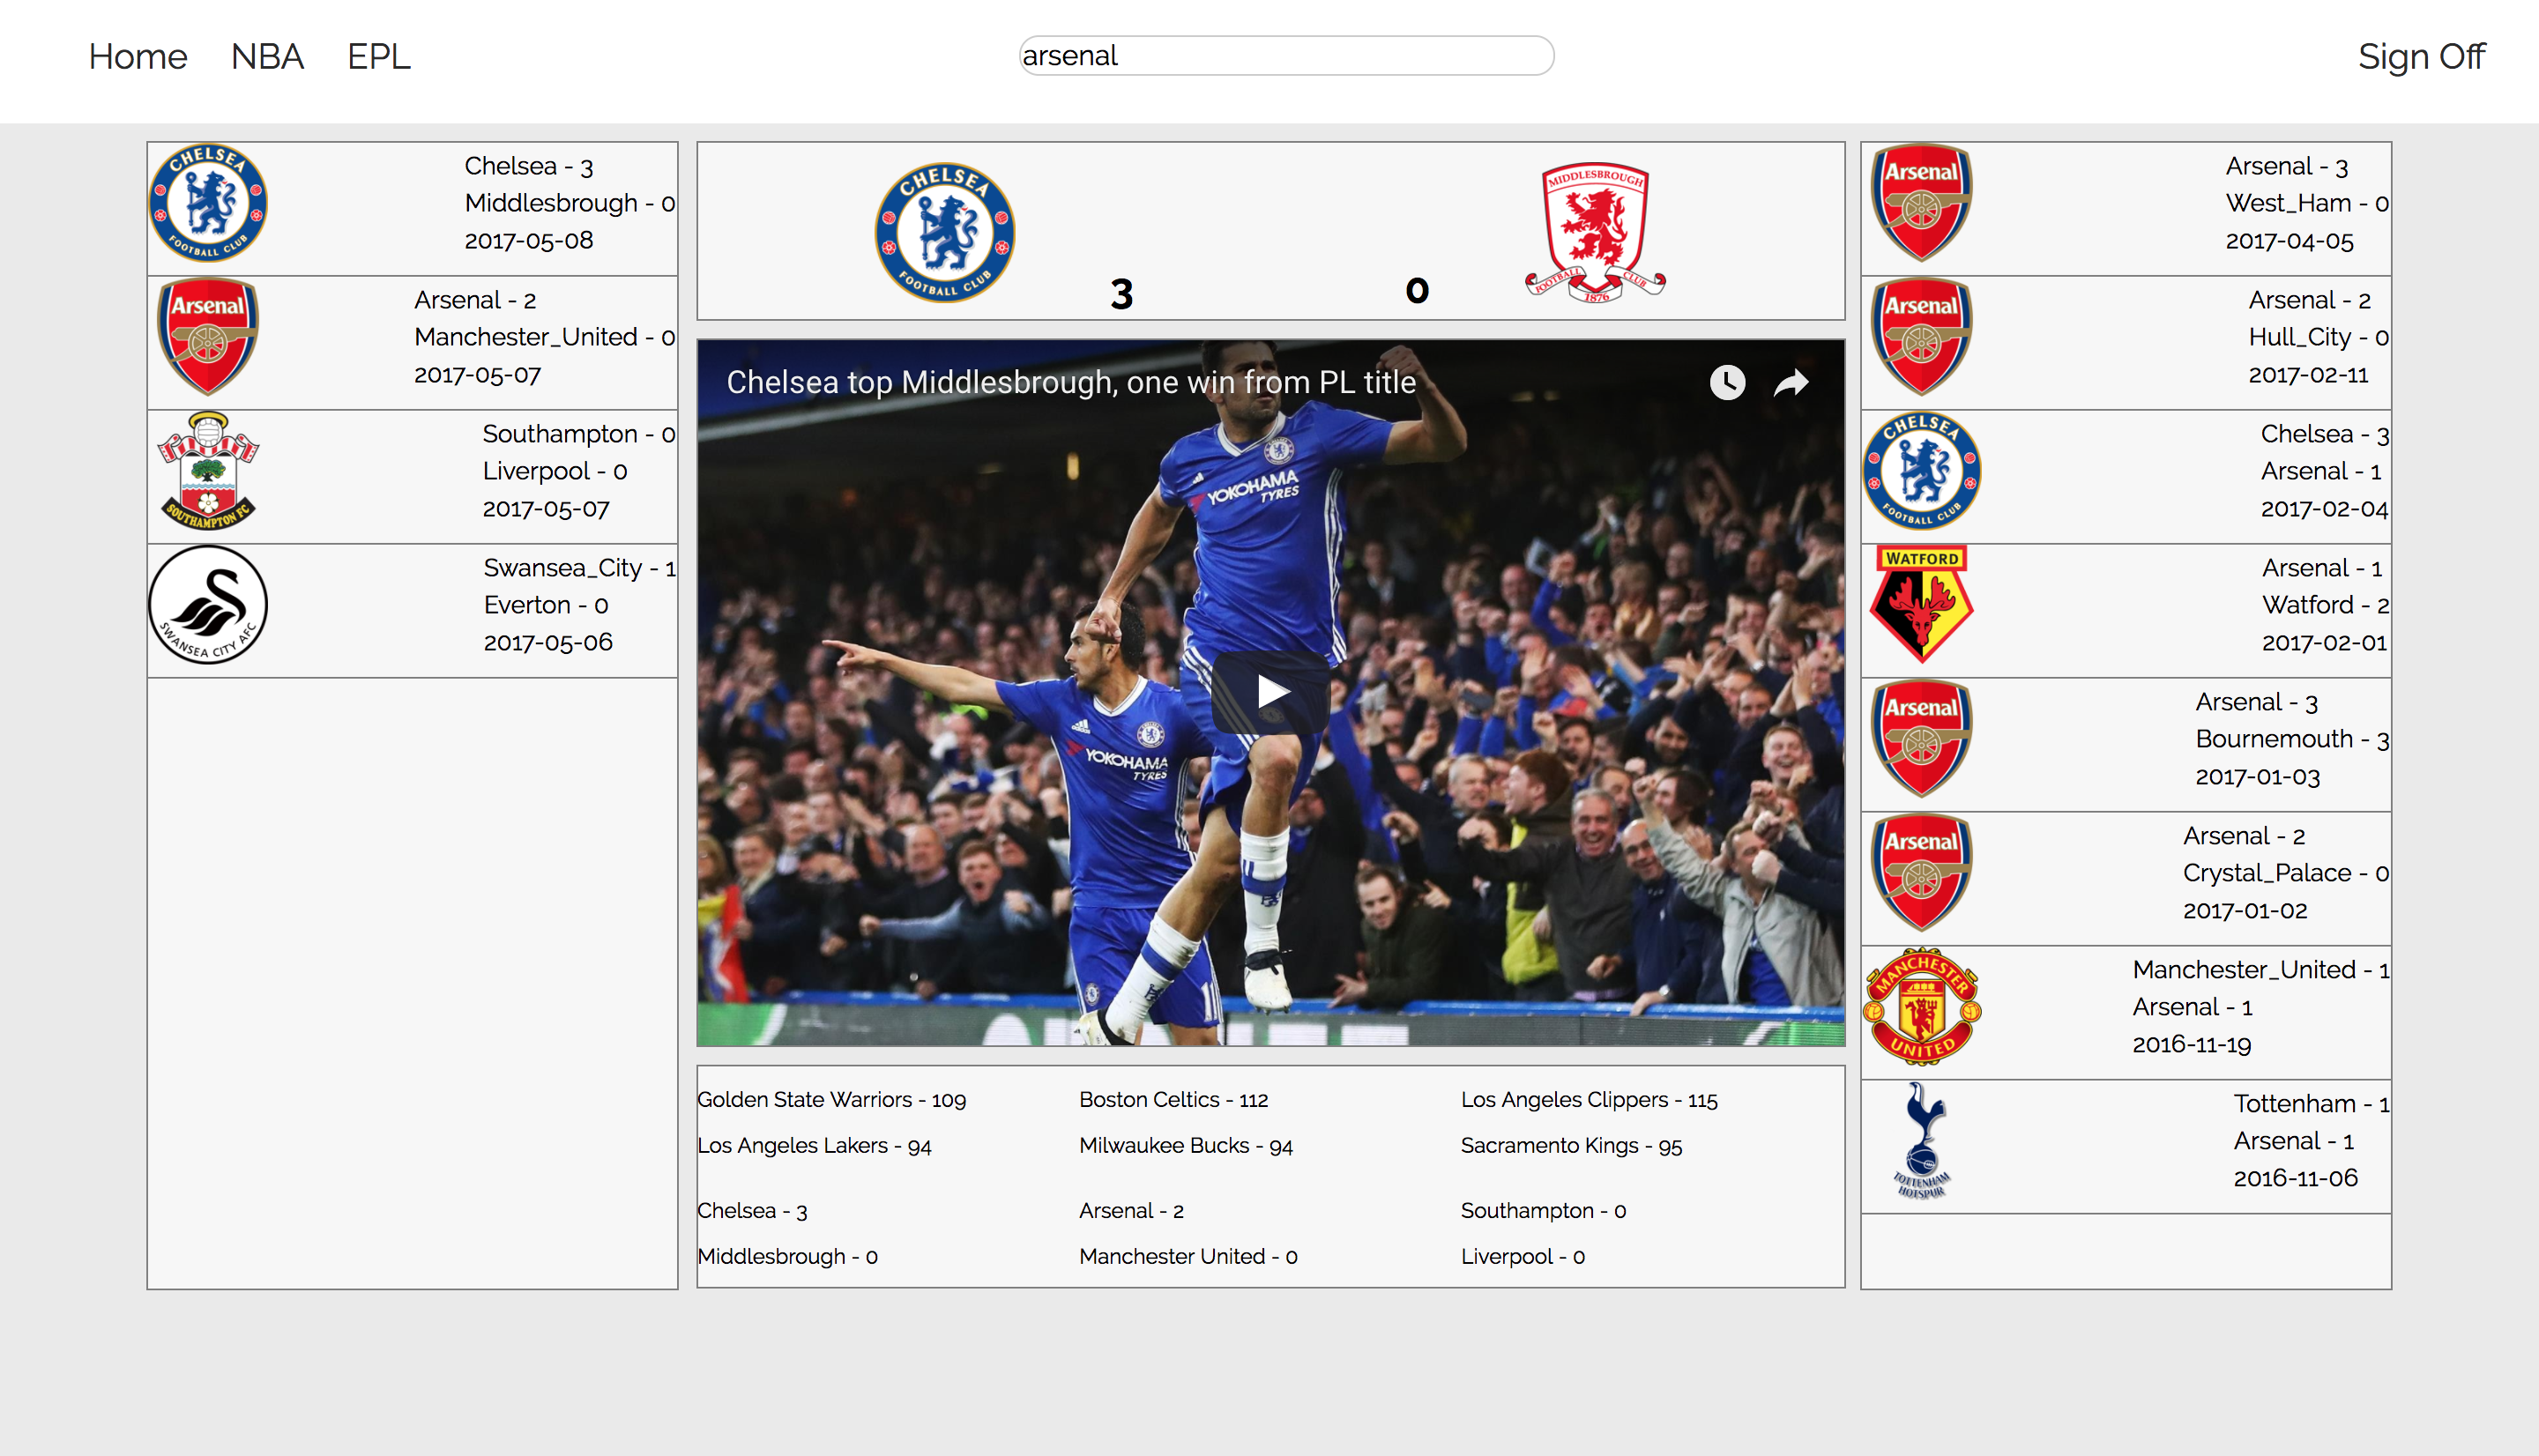
\includegraphics[scale=0.25]{loggedin.png}}
      \caption{Logged-In user on homepage}	
\end{figure}